\infolevone{
\subsection{Hodoscope}
The SHMS hodoscope consists of 4 planes, the first three made of bars
of scintillating plastic, and the fourth of synthetic quartz.  The
purposes of the hodoscope planes include, providing a trigger that is
approximately 100\% efficient for minimum ionizing particles, to
reject accidental coincidences in multi-arm experiments and to measure
the efficiency of the tracking system.

The first two planes of the hodoscope, S1X, and S1Y, are located
downstream of the second drift chamber.  The second two planes,
S2X and S2Y, are located about 2.2 meters downstream of the first pair.
The Heavy Gas Cherenkov and Aerogel Counter are located between
the hodoscope pairs.

\subsubsection{Scintillator Hodoscope Planes}
The SHMS scintillator planes are comprised of 13 paddles in S1X, 13
paddles in S1Y and 14 paddles in S2X.
Further information about the scintillator hodoscope planes
can be found in the ``SHMS Hodoscope Scintillator Detectors''
reference~\cite{howto:shms_scintillator_hodoscope}.
The scintillator material is
RP-408 from Rexon Corporation~\cite{rp408}.  Each paddle has a
photomultiplier tube on each end.  A mix of XP2262 and ET9214B tubes
are used.  The scintillator plane PMTs use negative high voltage.
Data sheets and testing information about these tubes and
their bases can be found in the Hall C document
database~\cite{docdb:XP2262docs,docdb:ET9214Bdocs}.

\subsubsection{Quartz Bar Hodoscope Plane}
The fourth plane of the SHMS hodoscope, S2Y,
(Figure~\ref{fig:quartzplane})
is comprised of 21 bars of Corning HPFS 7980 Fused Silica
\cite{corning} (quartz),
each with a length of 125 cm, width of 5.5 cm and thickness of 2.5 cm.
As the quartz only emits light from Cherenkov radiation, it is
relatively insensitive to low energy room backgrounds.  Each quartz
bar is read out by a photomultiplier at each end of the bar.  A mix
of Electron Tubes 9814Q, 9814W, and Photonis XP2020 tubes
are used.  All the
tubes are powered by positive high voltage through RB1102 (for
the 9814 tubes) and RB1106 (for the XP2020 tubes) resistive bases.
Data sheets, testing
and simulation information about these tubes and their bases can
be found in the Hall C document database~\cite{docdb:ET9814QBdocs}.

\begin{figure}
\begin{center}
  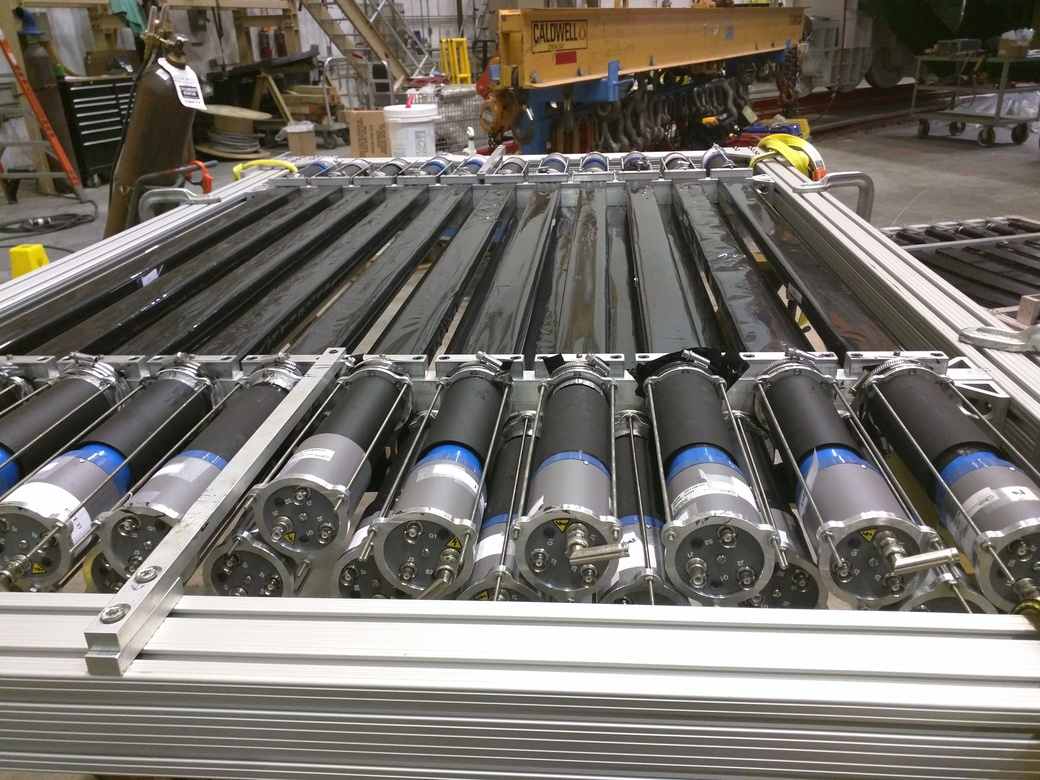
\includegraphics[width=.85\textwidth]{quartzplane.jpg}
  \caption{\label{fig:quartzplane}The SHMS quartz bar hodoscope plane, S2Y,
before mounting into the detector stack between S2X and the pre-shower
plane.}
\end{center}
\end{figure}

\subsubsection{Responsible Personnel}

The individuals responsible for the operation
of the hodoscopes are shown in Table \ref{tab:hod:personnel}.

\begin{namestab}{tab:hod:personnel}{Hodoscope responsible personnel}{%
      Hodoscope responsible personnel.}
  \DaveMack{}
%  \MahlonLong{}
  \GabrielNiculescu{Scintillator Planes}
  \IoanaNiculescu{Scintillator Planes}
  \AbdellahAhmidouch{Quartz Plane}
%  \SimonaMalace{}
\end{namestab}


}% \infolevone
